% Created by tikzDevice version 0.12.3.1 on 2021-10-16 19:49:33
% !TEX encoding = UTF-8 Unicode
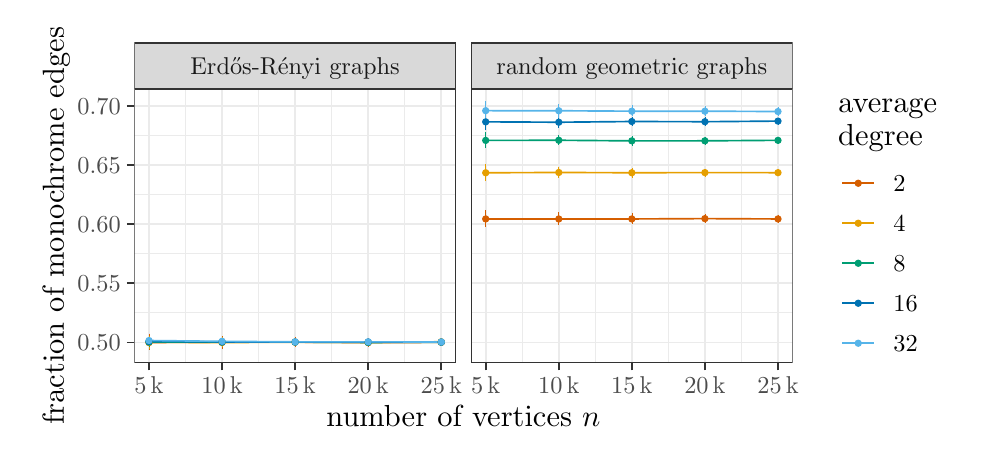
\begin{tikzpicture}[x=1pt,y=1pt]
\definecolor{fillColor}{RGB}{255,255,255}
\path[use as bounding box,fill=fillColor,fill opacity=0.00] (0,0) rectangle (339.67,151.77);
\begin{scope}
\path[clip] (  0.00,  0.00) rectangle (339.67,151.77);
\definecolor{drawColor}{RGB}{255,255,255}
\definecolor{fillColor}{RGB}{255,255,255}

\path[draw=drawColor,line width= 0.6pt,line join=round,line cap=round,fill=fillColor] (  0.00,  0.00) rectangle (339.67,151.77);
\end{scope}
\begin{scope}
\path[clip] ( 38.56, 30.69) rectangle (154.73,129.70);
\definecolor{fillColor}{RGB}{255,255,255}

\path[fill=fillColor] ( 38.56, 30.69) rectangle (154.73,129.70);
\definecolor{drawColor}{gray}{0.92}

\path[draw=drawColor,line width= 0.3pt,line join=round] ( 38.56, 48.75) --
	(154.73, 48.75);

\path[draw=drawColor,line width= 0.3pt,line join=round] ( 38.56, 70.12) --
	(154.73, 70.12);

\path[draw=drawColor,line width= 0.3pt,line join=round] ( 38.56, 91.49) --
	(154.73, 91.49);

\path[draw=drawColor,line width= 0.3pt,line join=round] ( 38.56,112.87) --
	(154.73,112.87);

\path[draw=drawColor,line width= 0.3pt,line join=round] ( 57.04, 30.69) --
	( 57.04,129.70);

\path[draw=drawColor,line width= 0.3pt,line join=round] ( 83.44, 30.69) --
	( 83.44,129.70);

\path[draw=drawColor,line width= 0.3pt,line join=round] (109.84, 30.69) --
	(109.84,129.70);

\path[draw=drawColor,line width= 0.3pt,line join=round] (136.24, 30.69) --
	(136.24,129.70);

\path[draw=drawColor,line width= 0.6pt,line join=round] ( 38.56, 38.06) --
	(154.73, 38.06);

\path[draw=drawColor,line width= 0.6pt,line join=round] ( 38.56, 59.43) --
	(154.73, 59.43);

\path[draw=drawColor,line width= 0.6pt,line join=round] ( 38.56, 80.81) --
	(154.73, 80.81);

\path[draw=drawColor,line width= 0.6pt,line join=round] ( 38.56,102.18) --
	(154.73,102.18);

\path[draw=drawColor,line width= 0.6pt,line join=round] ( 38.56,123.55) --
	(154.73,123.55);

\path[draw=drawColor,line width= 0.6pt,line join=round] ( 43.84, 30.69) --
	( 43.84,129.70);

\path[draw=drawColor,line width= 0.6pt,line join=round] ( 70.24, 30.69) --
	( 70.24,129.70);

\path[draw=drawColor,line width= 0.6pt,line join=round] ( 96.64, 30.69) --
	( 96.64,129.70);

\path[draw=drawColor,line width= 0.6pt,line join=round] (123.04, 30.69) --
	(123.04,129.70);

\path[draw=drawColor,line width= 0.6pt,line join=round] (149.45, 30.69) --
	(149.45,129.70);
\definecolor{drawColor}{RGB}{213,94,0}

\path[draw=drawColor,line width= 0.2pt,line join=round] ( 43.84, 41.18) --
	( 43.84, 41.18);

\path[draw=drawColor,line width= 0.2pt,line join=round] ( 43.84, 41.18) --
	( 43.84, 35.19);

\path[draw=drawColor,line width= 0.2pt,line join=round] ( 43.84, 35.19) --
	( 43.84, 35.19);

\path[draw=drawColor,line width= 0.2pt,line join=round] ( 70.24, 40.20) --
	( 70.24, 40.20);

\path[draw=drawColor,line width= 0.2pt,line join=round] ( 70.24, 40.20) --
	( 70.24, 35.73);

\path[draw=drawColor,line width= 0.2pt,line join=round] ( 70.24, 35.73) --
	( 70.24, 35.73);

\path[draw=drawColor,line width= 0.2pt,line join=round] ( 96.64, 40.06) --
	( 96.64, 40.06);

\path[draw=drawColor,line width= 0.2pt,line join=round] ( 96.64, 40.06) --
	( 96.64, 36.22);

\path[draw=drawColor,line width= 0.2pt,line join=round] ( 96.64, 36.22) --
	( 96.64, 36.22);

\path[draw=drawColor,line width= 0.2pt,line join=round] (123.04, 39.63) --
	(123.04, 39.63);

\path[draw=drawColor,line width= 0.2pt,line join=round] (123.04, 39.63) --
	(123.04, 36.40);

\path[draw=drawColor,line width= 0.2pt,line join=round] (123.04, 36.40) --
	(123.04, 36.40);

\path[draw=drawColor,line width= 0.2pt,line join=round] (149.45, 39.51) --
	(149.45, 39.51);

\path[draw=drawColor,line width= 0.2pt,line join=round] (149.45, 39.51) --
	(149.45, 36.61);

\path[draw=drawColor,line width= 0.2pt,line join=round] (149.45, 36.61) --
	(149.45, 36.61);
\definecolor{drawColor}{RGB}{230,159,0}

\path[draw=drawColor,line width= 0.2pt,line join=round] ( 43.84, 40.35) --
	( 43.84, 40.35);

\path[draw=drawColor,line width= 0.2pt,line join=round] ( 43.84, 40.35) --
	( 43.84, 35.56);

\path[draw=drawColor,line width= 0.2pt,line join=round] ( 43.84, 35.56) --
	( 43.84, 35.56);

\path[draw=drawColor,line width= 0.2pt,line join=round] ( 70.24, 39.84) --
	( 70.24, 39.84);

\path[draw=drawColor,line width= 0.2pt,line join=round] ( 70.24, 39.84) --
	( 70.24, 36.32);

\path[draw=drawColor,line width= 0.2pt,line join=round] ( 70.24, 36.32) --
	( 70.24, 36.32);

\path[draw=drawColor,line width= 0.2pt,line join=round] ( 96.64, 39.40) --
	( 96.64, 39.40);

\path[draw=drawColor,line width= 0.2pt,line join=round] ( 96.64, 39.40) --
	( 96.64, 36.67);

\path[draw=drawColor,line width= 0.2pt,line join=round] ( 96.64, 36.67) --
	( 96.64, 36.67);

\path[draw=drawColor,line width= 0.2pt,line join=round] (123.04, 39.23) --
	(123.04, 39.23);

\path[draw=drawColor,line width= 0.2pt,line join=round] (123.04, 39.23) --
	(123.04, 37.02);

\path[draw=drawColor,line width= 0.2pt,line join=round] (123.04, 37.02) --
	(123.04, 37.02);

\path[draw=drawColor,line width= 0.2pt,line join=round] (149.45, 39.25) --
	(149.45, 39.25);

\path[draw=drawColor,line width= 0.2pt,line join=round] (149.45, 39.25) --
	(149.45, 37.13);

\path[draw=drawColor,line width= 0.2pt,line join=round] (149.45, 37.13) --
	(149.45, 37.13);
\definecolor{drawColor}{RGB}{0,158,115}

\path[draw=drawColor,line width= 0.2pt,line join=round] ( 43.84, 40.11) --
	( 43.84, 40.11);

\path[draw=drawColor,line width= 0.2pt,line join=round] ( 43.84, 40.11) --
	( 43.84, 36.46);

\path[draw=drawColor,line width= 0.2pt,line join=round] ( 43.84, 36.46) --
	( 43.84, 36.46);

\path[draw=drawColor,line width= 0.2pt,line join=round] ( 70.24, 39.49) --
	( 70.24, 39.49);

\path[draw=drawColor,line width= 0.2pt,line join=round] ( 70.24, 39.49) --
	( 70.24, 36.95);

\path[draw=drawColor,line width= 0.2pt,line join=round] ( 70.24, 36.95) --
	( 70.24, 36.95);

\path[draw=drawColor,line width= 0.2pt,line join=round] ( 96.64, 39.15) --
	( 96.64, 39.15);

\path[draw=drawColor,line width= 0.2pt,line join=round] ( 96.64, 39.15) --
	( 96.64, 37.13);

\path[draw=drawColor,line width= 0.2pt,line join=round] ( 96.64, 37.13) --
	( 96.64, 37.13);

\path[draw=drawColor,line width= 0.2pt,line join=round] (123.04, 38.99) --
	(123.04, 38.99);

\path[draw=drawColor,line width= 0.2pt,line join=round] (123.04, 38.99) --
	(123.04, 37.14);

\path[draw=drawColor,line width= 0.2pt,line join=round] (123.04, 37.14) --
	(123.04, 37.14);

\path[draw=drawColor,line width= 0.2pt,line join=round] (149.45, 38.85) --
	(149.45, 38.85);

\path[draw=drawColor,line width= 0.2pt,line join=round] (149.45, 38.85) --
	(149.45, 37.33);

\path[draw=drawColor,line width= 0.2pt,line join=round] (149.45, 37.33) --
	(149.45, 37.33);
\definecolor{drawColor}{RGB}{0,114,178}

\path[draw=drawColor,line width= 0.2pt,line join=round] ( 43.84, 39.76) --
	( 43.84, 39.76);

\path[draw=drawColor,line width= 0.2pt,line join=round] ( 43.84, 39.76) --
	( 43.84, 37.04);

\path[draw=drawColor,line width= 0.2pt,line join=round] ( 43.84, 37.04) --
	( 43.84, 37.04);

\path[draw=drawColor,line width= 0.2pt,line join=round] ( 70.24, 39.10) --
	( 70.24, 39.10);

\path[draw=drawColor,line width= 0.2pt,line join=round] ( 70.24, 39.10) --
	( 70.24, 37.39);

\path[draw=drawColor,line width= 0.2pt,line join=round] ( 70.24, 37.39) --
	( 70.24, 37.39);

\path[draw=drawColor,line width= 0.2pt,line join=round] ( 96.64, 38.92) --
	( 96.64, 38.92);

\path[draw=drawColor,line width= 0.2pt,line join=round] ( 96.64, 38.92) --
	( 96.64, 37.46);

\path[draw=drawColor,line width= 0.2pt,line join=round] ( 96.64, 37.46) --
	( 96.64, 37.46);

\path[draw=drawColor,line width= 0.2pt,line join=round] (123.04, 38.84) --
	(123.04, 38.84);

\path[draw=drawColor,line width= 0.2pt,line join=round] (123.04, 38.84) --
	(123.04, 37.53);

\path[draw=drawColor,line width= 0.2pt,line join=round] (123.04, 37.53) --
	(123.04, 37.53);

\path[draw=drawColor,line width= 0.2pt,line join=round] (149.45, 38.75) --
	(149.45, 38.75);

\path[draw=drawColor,line width= 0.2pt,line join=round] (149.45, 38.75) --
	(149.45, 37.58);

\path[draw=drawColor,line width= 0.2pt,line join=round] (149.45, 37.58) --
	(149.45, 37.58);
\definecolor{drawColor}{RGB}{86,180,233}

\path[draw=drawColor,line width= 0.2pt,line join=round] ( 43.84, 39.94) --
	( 43.84, 39.94);

\path[draw=drawColor,line width= 0.2pt,line join=round] ( 43.84, 39.94) --
	( 43.84, 37.63);

\path[draw=drawColor,line width= 0.2pt,line join=round] ( 43.84, 37.63) --
	( 43.84, 37.63);

\path[draw=drawColor,line width= 0.2pt,line join=round] ( 70.24, 39.17) --
	( 70.24, 39.17);

\path[draw=drawColor,line width= 0.2pt,line join=round] ( 70.24, 39.17) --
	( 70.24, 37.75);

\path[draw=drawColor,line width= 0.2pt,line join=round] ( 70.24, 37.75) --
	( 70.24, 37.75);

\path[draw=drawColor,line width= 0.2pt,line join=round] ( 96.64, 38.86) --
	( 96.64, 38.86);

\path[draw=drawColor,line width= 0.2pt,line join=round] ( 96.64, 38.86) --
	( 96.64, 37.75);

\path[draw=drawColor,line width= 0.2pt,line join=round] ( 96.64, 37.75) --
	( 96.64, 37.75);

\path[draw=drawColor,line width= 0.2pt,line join=round] (123.04, 38.76) --
	(123.04, 38.76);

\path[draw=drawColor,line width= 0.2pt,line join=round] (123.04, 38.76) --
	(123.04, 37.74);

\path[draw=drawColor,line width= 0.2pt,line join=round] (123.04, 37.74) --
	(123.04, 37.74);

\path[draw=drawColor,line width= 0.2pt,line join=round] (149.45, 38.63) --
	(149.45, 38.63);

\path[draw=drawColor,line width= 0.2pt,line join=round] (149.45, 38.63) --
	(149.45, 37.79);

\path[draw=drawColor,line width= 0.2pt,line join=round] (149.45, 37.79) --
	(149.45, 37.79);
\definecolor{drawColor}{RGB}{213,94,0}

\path[draw=drawColor,line width= 0.6pt,line join=round] ( 43.84, 38.00) --
	( 70.24, 38.15) --
	( 96.64, 38.15) --
	(123.04, 37.97) --
	(149.45, 38.06);
\definecolor{drawColor}{RGB}{230,159,0}

\path[draw=drawColor,line width= 0.6pt,line join=round] ( 43.84, 38.10) --
	( 70.24, 37.98) --
	( 96.64, 38.13) --
	(123.04, 38.06) --
	(149.45, 38.27);
\definecolor{drawColor}{RGB}{0,158,115}

\path[draw=drawColor,line width= 0.6pt,line join=round] ( 43.84, 38.17) --
	( 70.24, 38.17) --
	( 96.64, 38.16) --
	(123.04, 38.02) --
	(149.45, 38.10);
\definecolor{drawColor}{RGB}{0,114,178}

\path[draw=drawColor,line width= 0.6pt,line join=round] ( 43.84, 38.40) --
	( 70.24, 38.20) --
	( 96.64, 38.17) --
	(123.04, 38.21) --
	(149.45, 38.17);
\definecolor{drawColor}{RGB}{86,180,233}

\path[draw=drawColor,line width= 0.6pt,line join=round] ( 43.84, 38.72) --
	( 70.24, 38.43) --
	( 96.64, 38.24) --
	(123.04, 38.24) --
	(149.45, 38.19);
\definecolor{drawColor}{RGB}{213,94,0}
\definecolor{fillColor}{RGB}{213,94,0}

\path[draw=drawColor,line width= 0.4pt,line join=round,line cap=round,fill=fillColor] ( 43.84, 38.00) circle (  1.11);

\path[draw=drawColor,line width= 0.4pt,line join=round,line cap=round,fill=fillColor] ( 70.24, 38.15) circle (  1.11);

\path[draw=drawColor,line width= 0.4pt,line join=round,line cap=round,fill=fillColor] ( 96.64, 38.15) circle (  1.11);

\path[draw=drawColor,line width= 0.4pt,line join=round,line cap=round,fill=fillColor] (123.04, 37.97) circle (  1.11);

\path[draw=drawColor,line width= 0.4pt,line join=round,line cap=round,fill=fillColor] (149.45, 38.06) circle (  1.11);
\definecolor{drawColor}{RGB}{230,159,0}
\definecolor{fillColor}{RGB}{230,159,0}

\path[draw=drawColor,line width= 0.4pt,line join=round,line cap=round,fill=fillColor] ( 43.84, 38.10) circle (  1.11);

\path[draw=drawColor,line width= 0.4pt,line join=round,line cap=round,fill=fillColor] ( 70.24, 37.98) circle (  1.11);

\path[draw=drawColor,line width= 0.4pt,line join=round,line cap=round,fill=fillColor] ( 96.64, 38.13) circle (  1.11);

\path[draw=drawColor,line width= 0.4pt,line join=round,line cap=round,fill=fillColor] (123.04, 38.06) circle (  1.11);

\path[draw=drawColor,line width= 0.4pt,line join=round,line cap=round,fill=fillColor] (149.45, 38.27) circle (  1.11);
\definecolor{drawColor}{RGB}{0,158,115}
\definecolor{fillColor}{RGB}{0,158,115}

\path[draw=drawColor,line width= 0.4pt,line join=round,line cap=round,fill=fillColor] ( 43.84, 38.17) circle (  1.11);

\path[draw=drawColor,line width= 0.4pt,line join=round,line cap=round,fill=fillColor] ( 70.24, 38.17) circle (  1.11);

\path[draw=drawColor,line width= 0.4pt,line join=round,line cap=round,fill=fillColor] ( 96.64, 38.16) circle (  1.11);

\path[draw=drawColor,line width= 0.4pt,line join=round,line cap=round,fill=fillColor] (123.04, 38.02) circle (  1.11);

\path[draw=drawColor,line width= 0.4pt,line join=round,line cap=round,fill=fillColor] (149.45, 38.10) circle (  1.11);
\definecolor{drawColor}{RGB}{0,114,178}
\definecolor{fillColor}{RGB}{0,114,178}

\path[draw=drawColor,line width= 0.4pt,line join=round,line cap=round,fill=fillColor] ( 43.84, 38.40) circle (  1.11);

\path[draw=drawColor,line width= 0.4pt,line join=round,line cap=round,fill=fillColor] ( 70.24, 38.20) circle (  1.11);

\path[draw=drawColor,line width= 0.4pt,line join=round,line cap=round,fill=fillColor] ( 96.64, 38.17) circle (  1.11);

\path[draw=drawColor,line width= 0.4pt,line join=round,line cap=round,fill=fillColor] (123.04, 38.21) circle (  1.11);

\path[draw=drawColor,line width= 0.4pt,line join=round,line cap=round,fill=fillColor] (149.45, 38.17) circle (  1.11);
\definecolor{drawColor}{RGB}{86,180,233}
\definecolor{fillColor}{RGB}{86,180,233}

\path[draw=drawColor,line width= 0.4pt,line join=round,line cap=round,fill=fillColor] ( 43.84, 38.72) circle (  1.11);

\path[draw=drawColor,line width= 0.4pt,line join=round,line cap=round,fill=fillColor] ( 70.24, 38.43) circle (  1.11);

\path[draw=drawColor,line width= 0.4pt,line join=round,line cap=round,fill=fillColor] ( 96.64, 38.24) circle (  1.11);

\path[draw=drawColor,line width= 0.4pt,line join=round,line cap=round,fill=fillColor] (123.04, 38.24) circle (  1.11);

\path[draw=drawColor,line width= 0.4pt,line join=round,line cap=round,fill=fillColor] (149.45, 38.19) circle (  1.11);
\definecolor{drawColor}{gray}{0.20}

\path[draw=drawColor,line width= 0.6pt,line join=round,line cap=round] ( 38.56, 30.69) rectangle (154.73,129.70);
\end{scope}
\begin{scope}
\path[clip] (160.23, 30.69) rectangle (276.40,129.70);
\definecolor{fillColor}{RGB}{255,255,255}

\path[fill=fillColor] (160.23, 30.69) rectangle (276.40,129.70);
\definecolor{drawColor}{gray}{0.92}

\path[draw=drawColor,line width= 0.3pt,line join=round] (160.23, 48.75) --
	(276.40, 48.75);

\path[draw=drawColor,line width= 0.3pt,line join=round] (160.23, 70.12) --
	(276.40, 70.12);

\path[draw=drawColor,line width= 0.3pt,line join=round] (160.23, 91.49) --
	(276.40, 91.49);

\path[draw=drawColor,line width= 0.3pt,line join=round] (160.23,112.87) --
	(276.40,112.87);

\path[draw=drawColor,line width= 0.3pt,line join=round] (178.71, 30.69) --
	(178.71,129.70);

\path[draw=drawColor,line width= 0.3pt,line join=round] (205.11, 30.69) --
	(205.11,129.70);

\path[draw=drawColor,line width= 0.3pt,line join=round] (231.51, 30.69) --
	(231.51,129.70);

\path[draw=drawColor,line width= 0.3pt,line join=round] (257.92, 30.69) --
	(257.92,129.70);

\path[draw=drawColor,line width= 0.6pt,line join=round] (160.23, 38.06) --
	(276.40, 38.06);

\path[draw=drawColor,line width= 0.6pt,line join=round] (160.23, 59.43) --
	(276.40, 59.43);

\path[draw=drawColor,line width= 0.6pt,line join=round] (160.23, 80.81) --
	(276.40, 80.81);

\path[draw=drawColor,line width= 0.6pt,line join=round] (160.23,102.18) --
	(276.40,102.18);

\path[draw=drawColor,line width= 0.6pt,line join=round] (160.23,123.55) --
	(276.40,123.55);

\path[draw=drawColor,line width= 0.6pt,line join=round] (165.51, 30.69) --
	(165.51,129.70);

\path[draw=drawColor,line width= 0.6pt,line join=round] (191.91, 30.69) --
	(191.91,129.70);

\path[draw=drawColor,line width= 0.6pt,line join=round] (218.31, 30.69) --
	(218.31,129.70);

\path[draw=drawColor,line width= 0.6pt,line join=round] (244.71, 30.69) --
	(244.71,129.70);

\path[draw=drawColor,line width= 0.6pt,line join=round] (271.12, 30.69) --
	(271.12,129.70);
\definecolor{drawColor}{RGB}{213,94,0}

\path[draw=drawColor,line width= 0.2pt,line join=round] (165.51, 85.78) --
	(165.51, 85.78);

\path[draw=drawColor,line width= 0.2pt,line join=round] (165.51, 85.78) --
	(165.51, 79.76);

\path[draw=drawColor,line width= 0.2pt,line join=round] (165.51, 79.76) --
	(165.51, 79.76);

\path[draw=drawColor,line width= 0.2pt,line join=round] (191.91, 85.13) --
	(191.91, 85.13);

\path[draw=drawColor,line width= 0.2pt,line join=round] (191.91, 85.13) --
	(191.91, 80.35);

\path[draw=drawColor,line width= 0.2pt,line join=round] (191.91, 80.35) --
	(191.91, 80.35);

\path[draw=drawColor,line width= 0.2pt,line join=round] (218.31, 84.81) --
	(218.31, 84.81);

\path[draw=drawColor,line width= 0.2pt,line join=round] (218.31, 84.81) --
	(218.31, 80.69);

\path[draw=drawColor,line width= 0.2pt,line join=round] (218.31, 80.69) --
	(218.31, 80.69);

\path[draw=drawColor,line width= 0.2pt,line join=round] (244.71, 84.49) --
	(244.71, 84.49);

\path[draw=drawColor,line width= 0.2pt,line join=round] (244.71, 84.49) --
	(244.71, 81.04);

\path[draw=drawColor,line width= 0.2pt,line join=round] (244.71, 81.04) --
	(244.71, 81.04);

\path[draw=drawColor,line width= 0.2pt,line join=round] (271.12, 84.18) --
	(271.12, 84.18);

\path[draw=drawColor,line width= 0.2pt,line join=round] (271.12, 84.18) --
	(271.12, 81.16);

\path[draw=drawColor,line width= 0.2pt,line join=round] (271.12, 81.16) --
	(271.12, 81.16);
\definecolor{drawColor}{RGB}{230,159,0}

\path[draw=drawColor,line width= 0.2pt,line join=round] (165.51,102.33) --
	(165.51,102.33);

\path[draw=drawColor,line width= 0.2pt,line join=round] (165.51,102.33) --
	(165.51, 96.43);

\path[draw=drawColor,line width= 0.2pt,line join=round] (165.51, 96.43) --
	(165.51, 96.43);

\path[draw=drawColor,line width= 0.2pt,line join=round] (191.91,101.44) --
	(191.91,101.44);

\path[draw=drawColor,line width= 0.2pt,line join=round] (191.91,101.44) --
	(191.91, 97.33);

\path[draw=drawColor,line width= 0.2pt,line join=round] (191.91, 97.33) --
	(191.91, 97.33);

\path[draw=drawColor,line width= 0.2pt,line join=round] (218.31,101.05) --
	(218.31,101.05);

\path[draw=drawColor,line width= 0.2pt,line join=round] (218.31,101.05) --
	(218.31, 97.61);

\path[draw=drawColor,line width= 0.2pt,line join=round] (218.31, 97.61) --
	(218.31, 97.61);

\path[draw=drawColor,line width= 0.2pt,line join=round] (244.71,100.83) --
	(244.71,100.83);

\path[draw=drawColor,line width= 0.2pt,line join=round] (244.71,100.83) --
	(244.71, 97.88);

\path[draw=drawColor,line width= 0.2pt,line join=round] (244.71, 97.88) --
	(244.71, 97.88);

\path[draw=drawColor,line width= 0.2pt,line join=round] (271.12,100.74) --
	(271.12,100.74);

\path[draw=drawColor,line width= 0.2pt,line join=round] (271.12,100.74) --
	(271.12, 98.06);

\path[draw=drawColor,line width= 0.2pt,line join=round] (271.12, 98.06) --
	(271.12, 98.06);
\definecolor{drawColor}{RGB}{0,158,115}

\path[draw=drawColor,line width= 0.2pt,line join=round] (165.51,113.91) --
	(165.51,113.91);

\path[draw=drawColor,line width= 0.2pt,line join=round] (165.51,113.91) --
	(165.51,108.44);

\path[draw=drawColor,line width= 0.2pt,line join=round] (165.51,108.44) --
	(165.51,108.44);

\path[draw=drawColor,line width= 0.2pt,line join=round] (191.91,112.99) --
	(191.91,112.99);

\path[draw=drawColor,line width= 0.2pt,line join=round] (191.91,112.99) --
	(191.91,109.30);

\path[draw=drawColor,line width= 0.2pt,line join=round] (191.91,109.30) --
	(191.91,109.30);

\path[draw=drawColor,line width= 0.2pt,line join=round] (218.31,112.68) --
	(218.31,112.68);

\path[draw=drawColor,line width= 0.2pt,line join=round] (218.31,112.68) --
	(218.31,109.14);

\path[draw=drawColor,line width= 0.2pt,line join=round] (218.31,109.14) --
	(218.31,109.14);

\path[draw=drawColor,line width= 0.2pt,line join=round] (244.71,112.34) --
	(244.71,112.34);

\path[draw=drawColor,line width= 0.2pt,line join=round] (244.71,112.34) --
	(244.71,109.46);

\path[draw=drawColor,line width= 0.2pt,line join=round] (244.71,109.46) --
	(244.71,109.46);

\path[draw=drawColor,line width= 0.2pt,line join=round] (271.12,112.22) --
	(271.12,112.22);

\path[draw=drawColor,line width= 0.2pt,line join=round] (271.12,112.22) --
	(271.12,109.83);

\path[draw=drawColor,line width= 0.2pt,line join=round] (271.12,109.83) --
	(271.12,109.83);
\definecolor{drawColor}{RGB}{0,114,178}

\path[draw=drawColor,line width= 0.2pt,line join=round] (165.51,120.41) --
	(165.51,120.41);

\path[draw=drawColor,line width= 0.2pt,line join=round] (165.51,120.41) --
	(165.51,114.77);

\path[draw=drawColor,line width= 0.2pt,line join=round] (165.51,114.77) --
	(165.51,114.77);

\path[draw=drawColor,line width= 0.2pt,line join=round] (191.91,119.84) --
	(191.91,119.84);

\path[draw=drawColor,line width= 0.2pt,line join=round] (191.91,119.84) --
	(191.91,115.64);

\path[draw=drawColor,line width= 0.2pt,line join=round] (191.91,115.64) --
	(191.91,115.64);

\path[draw=drawColor,line width= 0.2pt,line join=round] (218.31,119.47) --
	(218.31,119.47);

\path[draw=drawColor,line width= 0.2pt,line join=round] (218.31,119.47) --
	(218.31,116.09);

\path[draw=drawColor,line width= 0.2pt,line join=round] (218.31,116.09) --
	(218.31,116.09);

\path[draw=drawColor,line width= 0.2pt,line join=round] (244.71,119.31) --
	(244.71,119.31);

\path[draw=drawColor,line width= 0.2pt,line join=round] (244.71,119.31) --
	(244.71,116.35);

\path[draw=drawColor,line width= 0.2pt,line join=round] (244.71,116.35) --
	(244.71,116.35);

\path[draw=drawColor,line width= 0.2pt,line join=round] (271.12,119.25) --
	(271.12,119.25);

\path[draw=drawColor,line width= 0.2pt,line join=round] (271.12,119.25) --
	(271.12,116.71);

\path[draw=drawColor,line width= 0.2pt,line join=round] (271.12,116.71) --
	(271.12,116.71);
\definecolor{drawColor}{RGB}{86,180,233}

\path[draw=drawColor,line width= 0.2pt,line join=round] (165.51,125.20) --
	(165.51,125.20);

\path[draw=drawColor,line width= 0.2pt,line join=round] (165.51,125.20) --
	(165.51,118.34);

\path[draw=drawColor,line width= 0.2pt,line join=round] (165.51,118.34) --
	(165.51,118.34);

\path[draw=drawColor,line width= 0.2pt,line join=round] (191.91,124.06) --
	(191.91,124.06);

\path[draw=drawColor,line width= 0.2pt,line join=round] (191.91,124.06) --
	(191.91,119.29);

\path[draw=drawColor,line width= 0.2pt,line join=round] (191.91,119.29) --
	(191.91,119.29);

\path[draw=drawColor,line width= 0.2pt,line join=round] (218.31,123.77) --
	(218.31,123.77);

\path[draw=drawColor,line width= 0.2pt,line join=round] (218.31,123.77) --
	(218.31,119.69);

\path[draw=drawColor,line width= 0.2pt,line join=round] (218.31,119.69) --
	(218.31,119.69);

\path[draw=drawColor,line width= 0.2pt,line join=round] (244.71,123.34) --
	(244.71,123.34);

\path[draw=drawColor,line width= 0.2pt,line join=round] (244.71,123.34) --
	(244.71,119.81);

\path[draw=drawColor,line width= 0.2pt,line join=round] (244.71,119.81) --
	(244.71,119.81);

\path[draw=drawColor,line width= 0.2pt,line join=round] (271.12,123.03) --
	(271.12,123.03);

\path[draw=drawColor,line width= 0.2pt,line join=round] (271.12,123.03) --
	(271.12,119.85);

\path[draw=drawColor,line width= 0.2pt,line join=round] (271.12,119.85) --
	(271.12,119.85);
\definecolor{drawColor}{RGB}{213,94,0}

\path[draw=drawColor,line width= 0.6pt,line join=round] (165.51, 82.66) --
	(191.91, 82.64) --
	(218.31, 82.65) --
	(244.71, 82.77) --
	(271.12, 82.65);
\definecolor{drawColor}{RGB}{230,159,0}

\path[draw=drawColor,line width= 0.6pt,line join=round] (165.51, 99.34) --
	(191.91, 99.44) --
	(218.31, 99.35) --
	(244.71, 99.40) --
	(271.12, 99.37);
\definecolor{drawColor}{RGB}{0,158,115}

\path[draw=drawColor,line width= 0.6pt,line join=round] (165.51,111.03) --
	(191.91,111.08) --
	(218.31,110.87) --
	(244.71,110.88) --
	(271.12,111.06);
\definecolor{drawColor}{RGB}{0,114,178}

\path[draw=drawColor,line width= 0.6pt,line join=round] (165.51,117.74) --
	(191.91,117.60) --
	(218.31,117.86) --
	(244.71,117.79) --
	(271.12,118.01);
\definecolor{drawColor}{RGB}{86,180,233}

\path[draw=drawColor,line width= 0.6pt,line join=round] (165.51,121.78) --
	(191.91,121.75) --
	(218.31,121.59) --
	(244.71,121.59) --
	(271.12,121.47);
\definecolor{drawColor}{RGB}{213,94,0}
\definecolor{fillColor}{RGB}{213,94,0}

\path[draw=drawColor,line width= 0.4pt,line join=round,line cap=round,fill=fillColor] (165.51, 82.66) circle (  1.11);

\path[draw=drawColor,line width= 0.4pt,line join=round,line cap=round,fill=fillColor] (191.91, 82.64) circle (  1.11);

\path[draw=drawColor,line width= 0.4pt,line join=round,line cap=round,fill=fillColor] (218.31, 82.65) circle (  1.11);

\path[draw=drawColor,line width= 0.4pt,line join=round,line cap=round,fill=fillColor] (244.71, 82.77) circle (  1.11);

\path[draw=drawColor,line width= 0.4pt,line join=round,line cap=round,fill=fillColor] (271.12, 82.65) circle (  1.11);
\definecolor{drawColor}{RGB}{230,159,0}
\definecolor{fillColor}{RGB}{230,159,0}

\path[draw=drawColor,line width= 0.4pt,line join=round,line cap=round,fill=fillColor] (165.51, 99.34) circle (  1.11);

\path[draw=drawColor,line width= 0.4pt,line join=round,line cap=round,fill=fillColor] (191.91, 99.44) circle (  1.11);

\path[draw=drawColor,line width= 0.4pt,line join=round,line cap=round,fill=fillColor] (218.31, 99.35) circle (  1.11);

\path[draw=drawColor,line width= 0.4pt,line join=round,line cap=round,fill=fillColor] (244.71, 99.40) circle (  1.11);

\path[draw=drawColor,line width= 0.4pt,line join=round,line cap=round,fill=fillColor] (271.12, 99.37) circle (  1.11);
\definecolor{drawColor}{RGB}{0,158,115}
\definecolor{fillColor}{RGB}{0,158,115}

\path[draw=drawColor,line width= 0.4pt,line join=round,line cap=round,fill=fillColor] (165.51,111.03) circle (  1.11);

\path[draw=drawColor,line width= 0.4pt,line join=round,line cap=round,fill=fillColor] (191.91,111.08) circle (  1.11);

\path[draw=drawColor,line width= 0.4pt,line join=round,line cap=round,fill=fillColor] (218.31,110.87) circle (  1.11);

\path[draw=drawColor,line width= 0.4pt,line join=round,line cap=round,fill=fillColor] (244.71,110.88) circle (  1.11);

\path[draw=drawColor,line width= 0.4pt,line join=round,line cap=round,fill=fillColor] (271.12,111.06) circle (  1.11);
\definecolor{drawColor}{RGB}{0,114,178}
\definecolor{fillColor}{RGB}{0,114,178}

\path[draw=drawColor,line width= 0.4pt,line join=round,line cap=round,fill=fillColor] (165.51,117.74) circle (  1.11);

\path[draw=drawColor,line width= 0.4pt,line join=round,line cap=round,fill=fillColor] (191.91,117.60) circle (  1.11);

\path[draw=drawColor,line width= 0.4pt,line join=round,line cap=round,fill=fillColor] (218.31,117.86) circle (  1.11);

\path[draw=drawColor,line width= 0.4pt,line join=round,line cap=round,fill=fillColor] (244.71,117.79) circle (  1.11);

\path[draw=drawColor,line width= 0.4pt,line join=round,line cap=round,fill=fillColor] (271.12,118.01) circle (  1.11);
\definecolor{drawColor}{RGB}{86,180,233}
\definecolor{fillColor}{RGB}{86,180,233}

\path[draw=drawColor,line width= 0.4pt,line join=round,line cap=round,fill=fillColor] (165.51,121.78) circle (  1.11);

\path[draw=drawColor,line width= 0.4pt,line join=round,line cap=round,fill=fillColor] (191.91,121.75) circle (  1.11);

\path[draw=drawColor,line width= 0.4pt,line join=round,line cap=round,fill=fillColor] (218.31,121.59) circle (  1.11);

\path[draw=drawColor,line width= 0.4pt,line join=round,line cap=round,fill=fillColor] (244.71,121.59) circle (  1.11);

\path[draw=drawColor,line width= 0.4pt,line join=round,line cap=round,fill=fillColor] (271.12,121.47) circle (  1.11);
\definecolor{drawColor}{gray}{0.20}

\path[draw=drawColor,line width= 0.6pt,line join=round,line cap=round] (160.23, 30.69) rectangle (276.40,129.70);
\end{scope}
\begin{scope}
\path[clip] ( 38.56,129.70) rectangle (154.73,146.27);
\definecolor{drawColor}{gray}{0.20}
\definecolor{fillColor}{gray}{0.85}

\path[draw=drawColor,line width= 0.6pt,line join=round,line cap=round,fill=fillColor] ( 38.56,129.70) rectangle (154.73,146.27);
\definecolor{drawColor}{gray}{0.10}

\node[text=drawColor,anchor=base,inner sep=0pt, outer sep=0pt, scale=  0.88] at ( 96.64,134.95) {Erd{\H o}s-R\'enyi graphs};
\end{scope}
\begin{scope}
\path[clip] (160.23,129.70) rectangle (276.40,146.27);
\definecolor{drawColor}{gray}{0.20}
\definecolor{fillColor}{gray}{0.85}

\path[draw=drawColor,line width= 0.6pt,line join=round,line cap=round,fill=fillColor] (160.23,129.70) rectangle (276.40,146.27);
\definecolor{drawColor}{gray}{0.10}

\node[text=drawColor,anchor=base,inner sep=0pt, outer sep=0pt, scale=  0.88] at (218.31,134.95) {random geometric graphs};
\end{scope}
\begin{scope}
\path[clip] (  0.00,  0.00) rectangle (339.67,151.77);
\definecolor{drawColor}{gray}{0.20}

\path[draw=drawColor,line width= 0.6pt,line join=round] ( 43.84, 27.94) --
	( 43.84, 30.69);

\path[draw=drawColor,line width= 0.6pt,line join=round] ( 70.24, 27.94) --
	( 70.24, 30.69);

\path[draw=drawColor,line width= 0.6pt,line join=round] ( 96.64, 27.94) --
	( 96.64, 30.69);

\path[draw=drawColor,line width= 0.6pt,line join=round] (123.04, 27.94) --
	(123.04, 30.69);

\path[draw=drawColor,line width= 0.6pt,line join=round] (149.45, 27.94) --
	(149.45, 30.69);
\end{scope}
\begin{scope}
\path[clip] (  0.00,  0.00) rectangle (339.67,151.77);
\definecolor{drawColor}{gray}{0.30}

\node[text=drawColor,anchor=base,inner sep=0pt, outer sep=0pt, scale=  0.88] at ( 43.84, 19.68) {5\,k};

\node[text=drawColor,anchor=base,inner sep=0pt, outer sep=0pt, scale=  0.88] at ( 70.24, 19.68) {10\,k};

\node[text=drawColor,anchor=base,inner sep=0pt, outer sep=0pt, scale=  0.88] at ( 96.64, 19.68) {15\,k};

\node[text=drawColor,anchor=base,inner sep=0pt, outer sep=0pt, scale=  0.88] at (123.04, 19.68) {20\,k};

\node[text=drawColor,anchor=base,inner sep=0pt, outer sep=0pt, scale=  0.88] at (149.45, 19.68) {25\,k};
\end{scope}
\begin{scope}
\path[clip] (  0.00,  0.00) rectangle (339.67,151.77);
\definecolor{drawColor}{gray}{0.20}

\path[draw=drawColor,line width= 0.6pt,line join=round] (165.51, 27.94) --
	(165.51, 30.69);

\path[draw=drawColor,line width= 0.6pt,line join=round] (191.91, 27.94) --
	(191.91, 30.69);

\path[draw=drawColor,line width= 0.6pt,line join=round] (218.31, 27.94) --
	(218.31, 30.69);

\path[draw=drawColor,line width= 0.6pt,line join=round] (244.71, 27.94) --
	(244.71, 30.69);

\path[draw=drawColor,line width= 0.6pt,line join=round] (271.12, 27.94) --
	(271.12, 30.69);
\end{scope}
\begin{scope}
\path[clip] (  0.00,  0.00) rectangle (339.67,151.77);
\definecolor{drawColor}{gray}{0.30}

\node[text=drawColor,anchor=base,inner sep=0pt, outer sep=0pt, scale=  0.88] at (165.51, 19.68) {5\,k};

\node[text=drawColor,anchor=base,inner sep=0pt, outer sep=0pt, scale=  0.88] at (191.91, 19.68) {10\,k};

\node[text=drawColor,anchor=base,inner sep=0pt, outer sep=0pt, scale=  0.88] at (218.31, 19.68) {15\,k};

\node[text=drawColor,anchor=base,inner sep=0pt, outer sep=0pt, scale=  0.88] at (244.71, 19.68) {20\,k};

\node[text=drawColor,anchor=base,inner sep=0pt, outer sep=0pt, scale=  0.88] at (271.12, 19.68) {25\,k};
\end{scope}
\begin{scope}
\path[clip] (  0.00,  0.00) rectangle (339.67,151.77);
\definecolor{drawColor}{gray}{0.30}

\node[text=drawColor,anchor=base east,inner sep=0pt, outer sep=0pt, scale=  0.88] at ( 33.61, 35.03) {0.50};

\node[text=drawColor,anchor=base east,inner sep=0pt, outer sep=0pt, scale=  0.88] at ( 33.61, 56.40) {0.55};

\node[text=drawColor,anchor=base east,inner sep=0pt, outer sep=0pt, scale=  0.88] at ( 33.61, 77.78) {0.60};

\node[text=drawColor,anchor=base east,inner sep=0pt, outer sep=0pt, scale=  0.88] at ( 33.61, 99.15) {0.65};

\node[text=drawColor,anchor=base east,inner sep=0pt, outer sep=0pt, scale=  0.88] at ( 33.61,120.52) {0.70};
\end{scope}
\begin{scope}
\path[clip] (  0.00,  0.00) rectangle (339.67,151.77);
\definecolor{drawColor}{gray}{0.20}

\path[draw=drawColor,line width= 0.6pt,line join=round] ( 35.81, 38.06) --
	( 38.56, 38.06);

\path[draw=drawColor,line width= 0.6pt,line join=round] ( 35.81, 59.43) --
	( 38.56, 59.43);

\path[draw=drawColor,line width= 0.6pt,line join=round] ( 35.81, 80.81) --
	( 38.56, 80.81);

\path[draw=drawColor,line width= 0.6pt,line join=round] ( 35.81,102.18) --
	( 38.56,102.18);

\path[draw=drawColor,line width= 0.6pt,line join=round] ( 35.81,123.55) --
	( 38.56,123.55);
\end{scope}
\begin{scope}
\path[clip] (  0.00,  0.00) rectangle (339.67,151.77);
\definecolor{drawColor}{RGB}{0,0,0}

\node[text=drawColor,anchor=base,inner sep=0pt, outer sep=0pt, scale=  1.10] at (157.48,  7.64) {number of vertices $n$};
\end{scope}
\begin{scope}
\path[clip] (  0.00,  0.00) rectangle (339.67,151.77);
\definecolor{drawColor}{RGB}{0,0,0}

\node[text=drawColor,rotate= 90.00,anchor=base,inner sep=0pt, outer sep=0pt, scale=  1.10] at ( 13.08, 80.19) {fraction of monochrome edges};
\end{scope}
\begin{scope}
\path[clip] (  0.00,  0.00) rectangle (339.67,151.77);
\definecolor{fillColor}{RGB}{255,255,255}

\path[fill=fillColor] (287.40, 25.01) rectangle (334.17,135.37);
\end{scope}
\begin{scope}
\path[clip] (  0.00,  0.00) rectangle (339.67,151.77);
\definecolor{drawColor}{RGB}{0,0,0}

\node[text=drawColor,anchor=base west,inner sep=0pt, outer sep=0pt, scale=  1.10] at (292.90,121.23) {average};

\node[text=drawColor,anchor=base west,inner sep=0pt, outer sep=0pt, scale=  1.10] at (292.90,109.35) {degree};
\end{scope}
\begin{scope}
\path[clip] (  0.00,  0.00) rectangle (339.67,151.77);
\definecolor{fillColor}{RGB}{255,255,255}

\path[fill=fillColor] (292.90, 88.32) rectangle (307.35,102.78);
\end{scope}
\begin{scope}
\path[clip] (  0.00,  0.00) rectangle (339.67,151.77);
\definecolor{drawColor}{RGB}{213,94,0}

\path[draw=drawColor,line width= 0.2pt,line join=round] (294.34, 95.55) -- (305.91, 95.55);
\end{scope}
\begin{scope}
\path[clip] (  0.00,  0.00) rectangle (339.67,151.77);
\definecolor{drawColor}{RGB}{213,94,0}

\path[draw=drawColor,line width= 0.6pt,line join=round] (294.34, 95.55) -- (305.91, 95.55);
\end{scope}
\begin{scope}
\path[clip] (  0.00,  0.00) rectangle (339.67,151.77);
\definecolor{drawColor}{RGB}{213,94,0}
\definecolor{fillColor}{RGB}{213,94,0}

\path[draw=drawColor,line width= 0.4pt,line join=round,line cap=round,fill=fillColor] (300.12, 95.55) circle (  1.11);
\end{scope}
\begin{scope}
\path[clip] (  0.00,  0.00) rectangle (339.67,151.77);
\definecolor{fillColor}{RGB}{255,255,255}

\path[fill=fillColor] (292.90, 73.87) rectangle (307.35, 88.32);
\end{scope}
\begin{scope}
\path[clip] (  0.00,  0.00) rectangle (339.67,151.77);
\definecolor{drawColor}{RGB}{230,159,0}

\path[draw=drawColor,line width= 0.2pt,line join=round] (294.34, 81.10) -- (305.91, 81.10);
\end{scope}
\begin{scope}
\path[clip] (  0.00,  0.00) rectangle (339.67,151.77);
\definecolor{drawColor}{RGB}{230,159,0}

\path[draw=drawColor,line width= 0.6pt,line join=round] (294.34, 81.10) -- (305.91, 81.10);
\end{scope}
\begin{scope}
\path[clip] (  0.00,  0.00) rectangle (339.67,151.77);
\definecolor{drawColor}{RGB}{230,159,0}
\definecolor{fillColor}{RGB}{230,159,0}

\path[draw=drawColor,line width= 0.4pt,line join=round,line cap=round,fill=fillColor] (300.12, 81.10) circle (  1.11);
\end{scope}
\begin{scope}
\path[clip] (  0.00,  0.00) rectangle (339.67,151.77);
\definecolor{fillColor}{RGB}{255,255,255}

\path[fill=fillColor] (292.90, 59.42) rectangle (307.35, 73.87);
\end{scope}
\begin{scope}
\path[clip] (  0.00,  0.00) rectangle (339.67,151.77);
\definecolor{drawColor}{RGB}{0,158,115}

\path[draw=drawColor,line width= 0.2pt,line join=round] (294.34, 66.64) -- (305.91, 66.64);
\end{scope}
\begin{scope}
\path[clip] (  0.00,  0.00) rectangle (339.67,151.77);
\definecolor{drawColor}{RGB}{0,158,115}

\path[draw=drawColor,line width= 0.6pt,line join=round] (294.34, 66.64) -- (305.91, 66.64);
\end{scope}
\begin{scope}
\path[clip] (  0.00,  0.00) rectangle (339.67,151.77);
\definecolor{drawColor}{RGB}{0,158,115}
\definecolor{fillColor}{RGB}{0,158,115}

\path[draw=drawColor,line width= 0.4pt,line join=round,line cap=round,fill=fillColor] (300.12, 66.64) circle (  1.11);
\end{scope}
\begin{scope}
\path[clip] (  0.00,  0.00) rectangle (339.67,151.77);
\definecolor{fillColor}{RGB}{255,255,255}

\path[fill=fillColor] (292.90, 44.96) rectangle (307.35, 59.42);
\end{scope}
\begin{scope}
\path[clip] (  0.00,  0.00) rectangle (339.67,151.77);
\definecolor{drawColor}{RGB}{0,114,178}

\path[draw=drawColor,line width= 0.2pt,line join=round] (294.34, 52.19) -- (305.91, 52.19);
\end{scope}
\begin{scope}
\path[clip] (  0.00,  0.00) rectangle (339.67,151.77);
\definecolor{drawColor}{RGB}{0,114,178}

\path[draw=drawColor,line width= 0.6pt,line join=round] (294.34, 52.19) -- (305.91, 52.19);
\end{scope}
\begin{scope}
\path[clip] (  0.00,  0.00) rectangle (339.67,151.77);
\definecolor{drawColor}{RGB}{0,114,178}
\definecolor{fillColor}{RGB}{0,114,178}

\path[draw=drawColor,line width= 0.4pt,line join=round,line cap=round,fill=fillColor] (300.12, 52.19) circle (  1.11);
\end{scope}
\begin{scope}
\path[clip] (  0.00,  0.00) rectangle (339.67,151.77);
\definecolor{fillColor}{RGB}{255,255,255}

\path[fill=fillColor] (292.90, 30.51) rectangle (307.35, 44.96);
\end{scope}
\begin{scope}
\path[clip] (  0.00,  0.00) rectangle (339.67,151.77);
\definecolor{drawColor}{RGB}{86,180,233}

\path[draw=drawColor,line width= 0.2pt,line join=round] (294.34, 37.74) -- (305.91, 37.74);
\end{scope}
\begin{scope}
\path[clip] (  0.00,  0.00) rectangle (339.67,151.77);
\definecolor{drawColor}{RGB}{86,180,233}

\path[draw=drawColor,line width= 0.6pt,line join=round] (294.34, 37.74) -- (305.91, 37.74);
\end{scope}
\begin{scope}
\path[clip] (  0.00,  0.00) rectangle (339.67,151.77);
\definecolor{drawColor}{RGB}{86,180,233}
\definecolor{fillColor}{RGB}{86,180,233}

\path[draw=drawColor,line width= 0.4pt,line join=round,line cap=round,fill=fillColor] (300.12, 37.74) circle (  1.11);
\end{scope}
\begin{scope}
\path[clip] (  0.00,  0.00) rectangle (339.67,151.77);
\definecolor{drawColor}{RGB}{0,0,0}

\node[text=drawColor,anchor=base west,inner sep=0pt, outer sep=0pt, scale=  0.88] at (312.85, 92.52) {2};
\end{scope}
\begin{scope}
\path[clip] (  0.00,  0.00) rectangle (339.67,151.77);
\definecolor{drawColor}{RGB}{0,0,0}

\node[text=drawColor,anchor=base west,inner sep=0pt, outer sep=0pt, scale=  0.88] at (312.85, 78.07) {4};
\end{scope}
\begin{scope}
\path[clip] (  0.00,  0.00) rectangle (339.67,151.77);
\definecolor{drawColor}{RGB}{0,0,0}

\node[text=drawColor,anchor=base west,inner sep=0pt, outer sep=0pt, scale=  0.88] at (312.85, 63.61) {8};
\end{scope}
\begin{scope}
\path[clip] (  0.00,  0.00) rectangle (339.67,151.77);
\definecolor{drawColor}{RGB}{0,0,0}

\node[text=drawColor,anchor=base west,inner sep=0pt, outer sep=0pt, scale=  0.88] at (312.85, 49.16) {16};
\end{scope}
\begin{scope}
\path[clip] (  0.00,  0.00) rectangle (339.67,151.77);
\definecolor{drawColor}{RGB}{0,0,0}

\node[text=drawColor,anchor=base west,inner sep=0pt, outer sep=0pt, scale=  0.88] at (312.85, 34.71) {32};
\end{scope}
\end{tikzpicture}
